% This must be in the first 5 lines to tell arXiv to use pdfLaTeX, which is strongly recommended.
\pdfoutput=1
% In particular, the hyperref package requires pdfLaTeX in order to break URLs across lines.

\documentclass[11pt]{article}

% Remove the "review" option to generate the final version.
\usepackage[]{acl}
% Standard package includes
\usepackage{times}
\usepackage{latexsym}
% For proper rendering and hyphenation of words containing Latin characters (including in bib files)
\usepackage[T1]{fontenc}
% For Vietnamese characters
% \usepackage[T5]{fontenc}
% See https://www.latex-project.org/help/documentation/encguide.pdf for other character sets
% This assumes your files are encoded as UTF8
\usepackage[utf8]{inputenc}
% This is not strictly necessary, and may be commented out,
% but it will improve the layout of the manuscript,
% and will typically save some space.
\usepackage{float}
\usepackage{microtype}
\usepackage{enumitem}
\usepackage{geometry}
\geometry{margin=1in}  % Adjust this value as needed
\usepackage{tikz}
\usetikzlibrary{shapes.geometric, arrows.meta}

\tikzstyle{startstop} = [rectangle, rounded corners, minimum width=5cm, minimum height=1cm, text centered, draw=black, fill=white, font=\small]
\tikzstyle{arrow} = [thick,->,>=stealth]
% If the title and author information does not fit in the area allocated, uncomment the following
%
%\setlength\titlebox{<dim>}
%
% and set <dim> to something 5cm or larger.

\title{Chart-Aware Transformers: Learning Structured Embeddings for BI Report Understanding}

% Author information can be set in various styles:
% For several authors from the same institution:
% \author{Author 1 \and ... \and Author n \\
%         Address line \\ ... \\ Address line}
% if the names do not fit well on one line use
%         Author 1 \\ {\bf Author 2} \\ ... \\ {\bf Author n} \\
% For authors from different institutions:
% \author{Author 1 \\ Address line \\  ... \\ Address line
%         \And  ... \And
%         Author n \\ Address line \\ ... \\ Address line}
% To start a seperate ``row'' of authors use \AND, as in
% \author{Author 1 \\ Address line \\  ... \\ Address line
%         \AND
%         Author 2 \\ Address line \\ ... \\ Address line \And
%         Author 3 \\ Address line \\ ... \\ Address line}

\author{
\begin{tabular}{ccc}
\textbf{Akhil Srivatsava} & \textbf{Bimal Dev} & \textbf{Prashant Agarwal} \\
\texttt{sriakhil25@gmail.com} & \texttt{bimal.d3v@gmail.com} & \texttt{prashant.agarwal92@gmail.com} \\
\end{tabular}
}


\begin{document}

\maketitle

\section{Hypotheses} 

Traditional patch-based image tokenization methods, such as those employed in Vision Transformers (ViT), are sub-optimal for representing structured charts and BI reports, as they discard critical layout and semantic relationships inherent to chart elements.

We hypothesize that explicitly modeling chart elements - including titles, axes, legends, data marks (bars, lines, points), and annotations as discrete tokens, enriched with textual, semantic, and spatial (layout) embeddings, and processed through a Transformer encoder, will result in significantly more informative and semantically faithful representations for downstream tasks such as chart retrieval, question answering, and document understanding.

Specifically, we propose constructing chart element feature vectors containing attributes such as:

\begin{itemize}[noitemsep]
    \item Position (bounding box coordinates)
    \item Size (width and height)
    \item Type (bar, line, axis, title, etc.)
    \item Text content (labels and annotations)
    \item Visual attributes (color, thickness, style)
\end{itemize}

\section{Data}
For this experiment, we will use a combination of synthetic chart data, manually annotated images, and a publicly available chart dataset to train and evaluate our models.

The synthetic dataset will be generated using a variety of chart types, including bar charts, line charts, scatter plots, and others, with pixel-accurate COCO-style annotations for each chart element, such as bars, axis labels, legends, and tick marks. This synthetic dataset will provide a large and diverse set of chart images, enabling us to cover a broad range of possible scenarios and visual styles.

In addition to the synthetic data, we will also create a set of manually annotated images for training, ensuring high-quality, expert-level annotations for key chart elements. These images will be annotated following the COCO format, with bounding boxes for every relevant chart component, helping the model learn to detect and localize critical parts of the charts effectively.

For validation and evaluation, we will use the \textbf{ChartAssistant} dataset, publicly available on HuggingFace (\url{https://huggingface.co/datasets/FanqingM/ChartAssistant}). The ChartAssistant dataset provides a diverse collection of real-world and synthetic charts, paired with detailed annotations and natural language question-answer pairs. It covers a wide range of chart types, including bar charts, line charts, and pie charts, enabling us to rigorously assess the generalization ability of our model on realistic and complex chart understanding tasks.

Once fine-tuned, the trained Detectron2 model will be used to extract bounding boxes on new, previously unseen chart images. We will evaluate its performance across a wide range of chart types, styles, and visual variations to ensure robustness and scalability for real-world applications.


\section{Metrics} 
We will use a combination of quantitative and qualitative evaluation metrics to rigorously assess the effectiveness of our Chart-Aware Transformer model:

\subsection{Quantitative Metrics}

\subsubsection{Object Detection Performance (Detectron2 Stage)}

Since our first stage involves object detection:

\begin{itemize}
    \item \textbf{Mean Average Precision (mAP)}: Evaluate localization accuracy of bounding boxes for chart elements. Higher mAP indicates better localization and element identification capability.
    \item \textbf{Intersection-over-Union (IoU)}: Evaluate accuracy in localization. Common IoU threshold of 0.5 or 0.75 can be used for rigorous assessment.
\end{itemize}


\subsubsection{Retrieval Tasks (Element Embeddings)}

To measure quality of embeddings for retrieval tasks:

\begin{itemize}
    \item \textbf{Recall@K and Precision@K}: Measures how accurately and efficiently the correct charts are retrieved based on semantic queries.
    \item \textbf{Mean Reciprocal Rank (MRR)}: Evaluate ranking performance in retrieval scenarios.
\end{itemize}

\subsubsection{Chart Question Answering (QA Stage)}

For downstream chart understanding and reasoning tasks:

\begin{itemize}
    \item \textbf{Exact Match (EM)}: Strict metric measuring percentage of predictions matching the ground-truth exactly.
    \item \textbf{F1 Score}: Standard evaluation combining precision and recall to measure answer quality.
    \item \textbf{BLEU/ROUGE Scores} (optional): Useful if generating open-ended textual responses.
\end{itemize}

\subsection{Qualitative Metrics}

We plan qualitative analysis focusing on interpretability, robustness, and error diagnosis:

\begin{itemize}
    \item \textbf{Manual Error Analysis}: Review samples of incorrect predictions, categorizing common error patterns.
    \item \textbf{Embedding Visualization (t-SNE/PCA)}: Assess semantic coherence visually.
    \item \textbf{Case Studies}: Select representative examples to illustrate model strengths and weaknesses.
\end{itemize}

\section{Models} 
Our benchmarks will be based on a three-stage model inspired by insights from the UniChart, Chart Assistant, and Chart Instruct papers. The first stage focuses on bounding box extraction of chart elements using Detectron2, a high-performing object detection library built on top of Mask R-CNN. We are currently fine-tuning a Detectron2 model initialized with a ResNet-50 backbone pretrained on COCO, optimized for detecting chart-specific elements such as bars, lines, legends, and axes. Our fine-tuning process follows a supervised learning setup with COCO-style annotations, adapted to the chart data domain as described in UniChart.

Following detection, we plan to use an encoder model to convert the extracted bounding boxes and associated textual elements into dense embeddings. The specific encoder architecture is still under consideration. Inspired by Chart Instruct, we intend to train the encoder using contrastive learning objectives to ensure semantically related chart elements are close in embedding space.

In the final stage, we will use a decoder model that takes the generated embeddings along with a user's natural language question as input, and outputs a structured answer. We are exploring sequence-to-sequence (seq2seq) models and transformer-based decoders for this purpose, aiming to align the decoder training with the chart reasoning objectives discussed in Chart Assistant.

\begin{figure}[H]
\centering
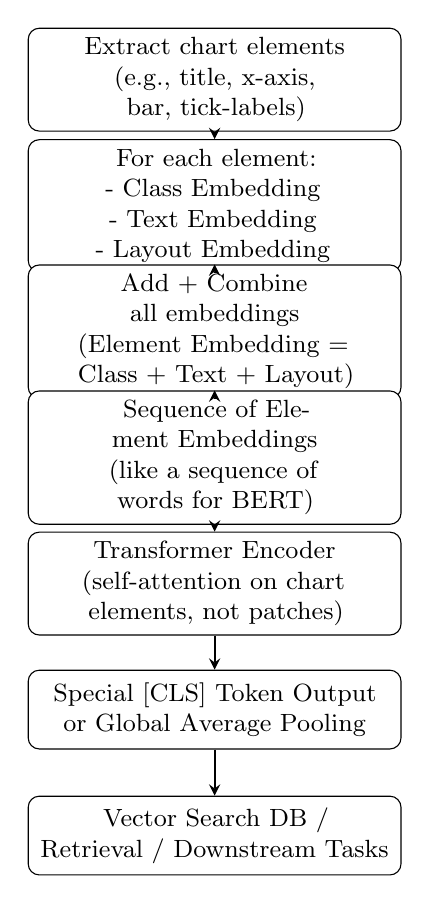
\begin{tikzpicture}[scale=0.8]
% Define styles inside the environment
\tikzset{
  box/.style={rectangle, draw, rounded corners, fill=white, 
              text width=4.5cm, minimum height=1cm, align=center, font=\small},
  arrow/.style={->, >=stealth, thick}
}

% Nodes - simple boxes with fixed positions
\node[box] (start) at (0,0) {Extract chart elements \\ (e.g., title, x-axis, bar, tick-labels)};
\node[box] (element) at (0,-2) {For each element:\\- Class Embedding \\- Text Embedding \\- Layout Embedding};
\node[box] (combine) at (0,-4) {Add + Combine all embeddings \\ (Element Embedding = Class + Text + Layout)};
\node[box] (sequence) at (0,-6) {Sequence of Element Embeddings \\ (like a sequence of words for BERT)};
\node[box] (transformer) at (0,-8) {Transformer Encoder \\ (self-attention on chart elements, not patches)};
\node[box] (output) at (0,-10) {Special [CLS] Token Output \\ or Global Average Pooling};
\node[box] (downstream) at (0,-12) {Vector Search DB / \\ Retrieval / Downstream Tasks};

% Simple straight arrows
\draw[arrow] (start) -- (element);
\draw[arrow] (element) -- (combine);
\draw[arrow] (combine) -- (sequence);
\draw[arrow] (sequence) -- (transformer);
\draw[arrow] (transformer) -- (output);
\draw[arrow] (output) -- (downstream);

\end{tikzpicture}
\caption{High-level architecture of the Chart-Aware Transformer.}
\label{fig:chart_transformer}
\end{figure}

\section{General Reasoning}

To support our hypothesis, we first construct a detailed annotated dataset by extracting fine-grained components from charts, such as titles, axes, tick labels, bars, lines, and legends. Using Matplotlib, we generate bounding box annotations in a controlled synthetic environment. We then fine-tune Detectron2 on these annotated charts to generalize detection to varied chart styles and visual designs, enabling scalable automatic labeling. These structured annotations serve as input to our proposed Chart-Aware Transformer, modeling relationships between elements rather than pixel patches. Thus, our pipeline directly tests the hypothesis that element-level understanding significantly enhances accuracy, interpretability, and generalizability in chart comprehension.

\section{Summary of Progress}
We have generated synthetic datasets, begun manual annotations, and initiated Detectron2 fine-tuning. Next steps include embedding model selection, decoder implementation, and integration. Potential challenges include GPU constraints and embedding convergence.

\appendix
% Entries for the entire Anthology, followed by custom entries
\nocite{bendeck2024gpt4vis, masry2023unichart, chartassistant_dataset, huang2023layoutlmv3, huang2024survey, li2024visualizationliteracy, liu2023vectordbsurvey, lin2024chartinstruct, zhang2024chartassistant, zhang2024mmgem}

\bibliographystyle{acl_natbib}
\bibliography{anthology,custom}

\end{document}